%!TEX root = ../Masterthesis.tex
\chapter{System conception}\section{Technical conception}
\begin{figure}[H]
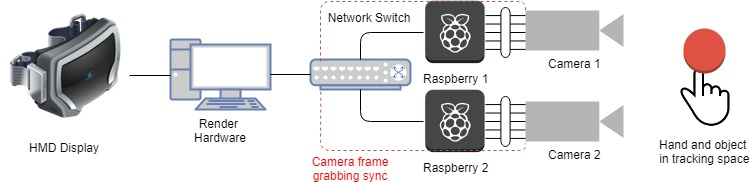
\includegraphics[width=\textwidth]{images/technical_setup.jpg}
\caption{Technical conception of the single hardware parts}
\label{technical-copnception}
\end{figure} 
The technical setup of the whole system is relatively simple. Instead of using one large dimensioned unit which takes care of all calculations, the image processing steps that have to be done on both stereo images anyway, are outsourced onto the Raspberry Pis. 
\todo{rewrite}As already mentioned in the conception phase, the image processing done directly on the Pi also reduces latency.This  would occur when sending image data over network channels to the main unit.\\
The two \textbf{Raspberry Pi 3 Model B}, which are used as the controllers for the \textbf{Raspberry Pi Camera} are connected via network cable to a network switch. A connection over wireless network would be possible with the on-board capabilities, but this might create latency problems and/or signal interference with other existing networks. Therefor a cable connection is the safer solution.
The switch also connects to the "Master" PC to which the "Slave" Pi's communicate their data. The Master also takes care of the stereoscopic calculations,as it is dimensioned with far more computational power than the slaves. The 2D positional data from the slaves and the calculation results from the stereo image disparity is fed into the hand model running on the "Master". The model solution is then applied to the digital hand model and rendered to the HMD.
\section{Image Analysis with OpenCV 3 and Python on the Raspberry}
For the image analysis part, \textit{OpenCV3} with it's \textit{Python 3} bindings is chosen. The \textit{OpenCV} package needs to be downloaded and compiled onto each device before it can be used.
Before the actual image analysis part can take place, the used cameras need to be calibrated. As they are basically pinhole cameras, they introduce amounts of radial and tangential distortion to the images. These distortions need to be compensated for, especially when using them as source for the stereo images. Image distortion in these pictures would lead to incorrect calculations for image depth.
\textit{OpenCV} supplies the tools to calculate the distortion parameters as well as the camera matrix \cite{Opencv.2018}.
The camera matrix is basically a description for the transformation of points in 3D object space to the 2D image space of the camera. For the used Cameras, we can consider a central projection of points in space onto our image plane. The center of the camera is considered the center of an euclidean coordinate system and the projection plane \textbf{z} is located at distance \textit{f} equal to the focal length of the camera.\\
\begin{figure}[H]
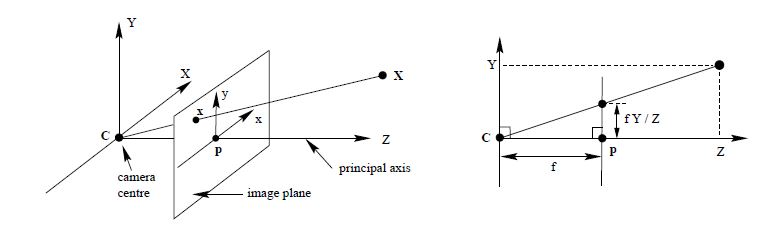
\includegraphics[width=\textwidth]{images/pionhole.JPG}
\caption{Image point projection for pinhole camera systems\cite{Hartley.2000}}
\label{pinholecamera_mapping} 
\end{figure}
As shown in Figure \ref{pinholecamera_mapping}, a point from the object space can be projected onto the image plane by drawing a ray from the object space point to the camera center. The intersection point of the ray with the image plane defines the projection point. With this knowledge the projection can be described as :
\begin{equation}
(X,Y,Z)^{T} \mapsto (fX/Z,fY/Z)^{T}
\end{equation}
\todo {elaborate}

For the calculation of the image distortion , \textit{OpenCv} uses a chessboard image for calibration. The printed image is held in front of the camera at a constant distance and rotated and positioned differently. After every position/rotation change an image of the pattern should be taken.
These images are then used to find the corners at the intersection of the black and white squares. With the previous knowledge of the square sizes, the projection errors in radial and tangential directions can be calculated:\todo{add Source code}
\begin{equation}
\begin{split}
x_{tanDistorted}&=x(1+k_{1}r^{2}+k_{2}r^{4}+k_{3}+r^{6})\\
y_{tanDistorted}&=y(1+k_{1}r^{2}+k_{2}r^{4}+k_{3}+r^{6})\\
\\
x_{radDistorted}&=x+[2p_{1}xy+p_{2}(r^{2}+2x^{2})]\\
y_{radDistorted}&=x+[p_{1}(r^{2}+2y^{2})+2p_{2}xy]\\
\end{split}
\end{equation} 
As can bee seen from the above equations, the parameters that need to be calculated are $k_{1},k_{2},p_{1},p_{2},k_{3}$.
\todo{continue}

The python program prototype that is used for tracking the specified color markers is comprised of the following components:
\begin{itemize}
\item Image acquisition from camera
\item Image conversion to HSV colorspace
\item Mask construction and Filtering
\item Contour finding an position calculation
\item Sending of positional data via Network as UPD Package
\end{itemize}

\subsection{Image acquisition from camera}
As the computation times for image filtering and mask generation may vary, it makes sense to separate the image acquisition from the computation part.Therefore the loading of the image data frame from the camera is outsourced into its own thread. Also this allows us to trigger the frame grabbing on both devices for synchronization. Frame grabbing synchronization can be done via triggering a PWM signal on one of the raspberry's and sending it to the other Pi.
The synchronicity of the two frame reading threads is assumed for the first implementation and has to be tested on a finished setup.\\
The tread takes the data of the current image frame and hands it over to the main thread, where the image processing is handled. For the first frames, the full image data is needed as the position of the markers is not yet known. Performance-wise, this introduces a lot of overhead, since each mask generation step for the specific colors hast to go through the complete image data, meaning every pixel has to be read out at least 5 times to get the tracking for all different markers.\\
\begin{figure}[H]
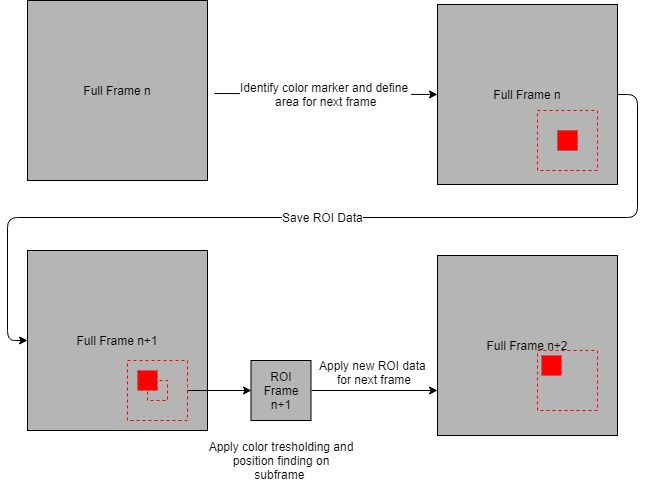
\includegraphics[width=\textwidth]{images/ROI.jpg}
\caption{ROI calculation for consecutive frames}
\label{roi_calc} 
\end{figure}
After a few frames, we get hold of the marker position and can define a reduced region of interest (ROI) on the image (Figure \ref{roi_calc}). The new ROI results from the positional data of the previous frame and has to be dimensioned correctly as to incorporate the possibility of large position differences between consecutive frames.\\
Furthermore the offset position, preferably the top left corner of the region, has to be kept track of. By taking a sub-region of the frame as input for further processing, the resulting coordinates relate to the top left corner of this sub-region as origin. Consequently only the first set of coordinates has the correct origin as reference point for the next frame. Consecutive frames need this information to retrieve the correct sub-region from the full frame by adding the offset to the calculated positional data.
First frame ROI calculation is based on a minimum axis-aligned bounding box(AABB) fitted onto the marker. The offset value for the ROI is added to the bounding box values resulting in a rectangle data-set containing the position of the offset top-left corner $\vec{\mathbf{tl}}$ and the offset 
\textbf{width} and \textbf{height} of the ROI rectangle:
\begin{equation}
\begin{split}
\vec{\mathbf{tl_{0}}}&=(AABB_{x_{0}}-\text{offset}_{x},AABB_{y_{0}}-\text{offset}_{y})\\
\mathbf{width}&=AABB{w_{0}}+(2\cdot\text{offset}_{x})\\
\mathbf{height}&=AABB_{h_{0}}+(2\cdot\text{offset}_{y})\\
\end{split}
\end{equation}
These values are taken to extract the sub-region of the consecutive at $\vec{\mathbf{tl}}$ with size of width and height. The $\vec{\mathbf{tl}}$ value is also saved as offset value $\vec{\mathbf{OffPos}}$ .
The position calculation for the proximate frame will utilize the offset value as follows:
\begin{equation}
\begin{split}
\vec{\mathbf{tl_{1}}_{x}}&=x_{1}+\vec{\mathbf{OffPos}}_{x}-\text{offset}_{x} \\ \vec{\mathbf{tl_{1}}_{y}}&=y_{1}+\vec{\mathbf{OffPos}}_{y}-\text{offset}_{y}\\
\mathbf{width}&=AABB_{w_{1}}+(2\cdot\text{offset}_{x})\\
\mathbf{height}&=AABB_{h_{1}}+(2\cdot\text{offset}_{y})\\
\end{split}
\end{equation}
This should result in the correct positional data for all frames following the initial frame.
Finally,the resulting rectangle has to be fitted onto the size boundaries of the full image frame. When applying a fixed offset value, the resulting region that will be extracted from the following frame might reach outside the size boundaries of the full frame. This can happen when the markers are positioned near the edges of the frame. Trying to read out pixels outside the available size of the image will without doubt result into an error by reason of unavailable data at these points. Therefore the combination of position width, height and offset has to be clamped to fit into the available image data:
\begin{equation}
\begin{split}
\textbf{width}&=\text(max(0,min(\mathbf{width},image_{width}))\\
\textbf{height}&=\text(max(0,min(\mathbf{height},image_{height}))
\end{split}
\end{equation}
Another option which could be evaluated instead of clamping the area would be shifting the offset point to a position where it does not violate the image boundaries and  thereby preserving the size of the ROI.\\
Should no marker be found in the defined ROI or the certainty of the result is not high enough, the frame has to be dropped and the next frame should utilize the whole image data.
\subsection{Image conversion to HSV colorspace}
The image data that is supplied by the camera comes in an RGB data format, which we could already use for the further calculation. It does though make more sense to convert the input data into the HSV colorspace. Since we are not using high precision cameras, it is necessary to define a range of color values around the desired color which we want to track. The HSV colorspace is displayed as a cone, in comparison to the RGB colorspace, which is displayed as a cube. The color values for the HSV space are all located on a circle spanning form 0 to 360 degrees. The Hue value (H)corresponds to the angle on the circle, where $0^\circ$ corresponds to a reddish color, $120^\circ$ lies in the area of green and $240^\circ$ and above correspond to blue. The saturation value (s) corresponds to the amount of white the color contains  where 0 is pure white and 100 corresponds to the fully saturated color. For optimal results, only highly saturated colors should be used to ensure correct color detection. The last component is the value component (V) which describes the intensity of the color. Alike the value settings for the saturation, value ranges of at leas 50 should be used for tracking precision.
\\
For tracking the five fingers of the hand we need five distinguishable colors. Here the primary colors red, green and blue will be the choice for the first three colors. The other two selected colors \todo {check test results} are orange and yellow. To be able to clearly distinguish these colors in the video frame, a constant and homogeneous lighting is needed as well as a color temperature of the lighting that is in the neutral area to not change the color of the markers.
\\the color conversion from the input RGB values to the desired HSV colorspace is done as follows:
\begin{equation}
\begin{split}
hsv_{low}=(hue_{targetcolor}-sensitivity,100,100)\\
hsv_{up}=(hue_{targetcolor}-sensitivity,100,100)\\
\end{split}
\end{equation}
\subsection{Mask construction and filtering}
\todo {orig image and mask images for display}
These values are the used as the parameters for a mask generation which generates a binary mask for the current frame where all pixels whose values lie outside of the specified range are set to zero (black) and the remaining are set to 255 (white).For these masks to work properly, any other larger objects that might contain similar colors should be removed from the scene to eliminate wrong tracking data. The used cameras run on an automated white balance and exposure mode. The variation of these values can cause shifts in the appearance of the colored markers and therefore alter the generated masks. To compensate for white balance shifting, a non-white ideally diffuse reflecting background should be used for the tracking space. Also the auto modes should be turned off and appropriate values for white balance and exposure have to be determined at the initialization step of the system.\\As all digital cameras tend to have signal noise in the sensor data , high frequency  noise in the color channels will be present. This noise should be filtered out before any further computation on the image data can be done.\\
The first step in this progress is to use a Gaussian filter to blur the mask.
The Gaussian filter acts as a low pass filter for the image. The application of the filter cuts out high frequency noise generated by the sensor electronic and other factors. The downside of applying a Blur onto the generated image is a loss of detail. As the markers will not be utilizing complex geometric forms or fine patterns, the loss of details is acceptable.\\After this step an erosion and a dilation is applied to the image tho further eliminate unwanted noise. A combination of these two morphological operation  is used to further improve the data of the thresholded binary image\cite[chapter~3.11-12]{Davies.2017}.\todo {elaborate}.
Erosion and dilation operation on thresholded images perform the tasks of removing light spots on dark backgrounds as well as dark spots on light backgrounds. These spots are normaly the result of the remaining image noise after the blurring or incorrect pixel values from the camera which case the pixel to be incorrectly thresholded.



\subsection{Contour finding and position calculation}
With the cleaned mask we can continue and search for the white areas in the mask which might represent our target. Under the assumption that we have removed all other parasitic objects from the image, the marker should be the largest area of positive pixels in the mask frame. Therefore only the largest area found in the search is taken as the desired tracking marker. For the selected area, a fitting bounding box is calculated and the center of this box is used as the positional parameter of the tracking marker.
\subsection{Sending of positional data via network as UPD package}
The resulting data is then handed over to a UDP server which sends the positional data to the parent device where the stereoscopic calculations as well as the hand model and rendering is done
\subsection{object tracking}
\todo{add object tracking method -> visual or HTC vive tracker}
 



 




